


\tikzset{every picture/.style={line width=0.75pt}} %set default line width to 0.75pt        

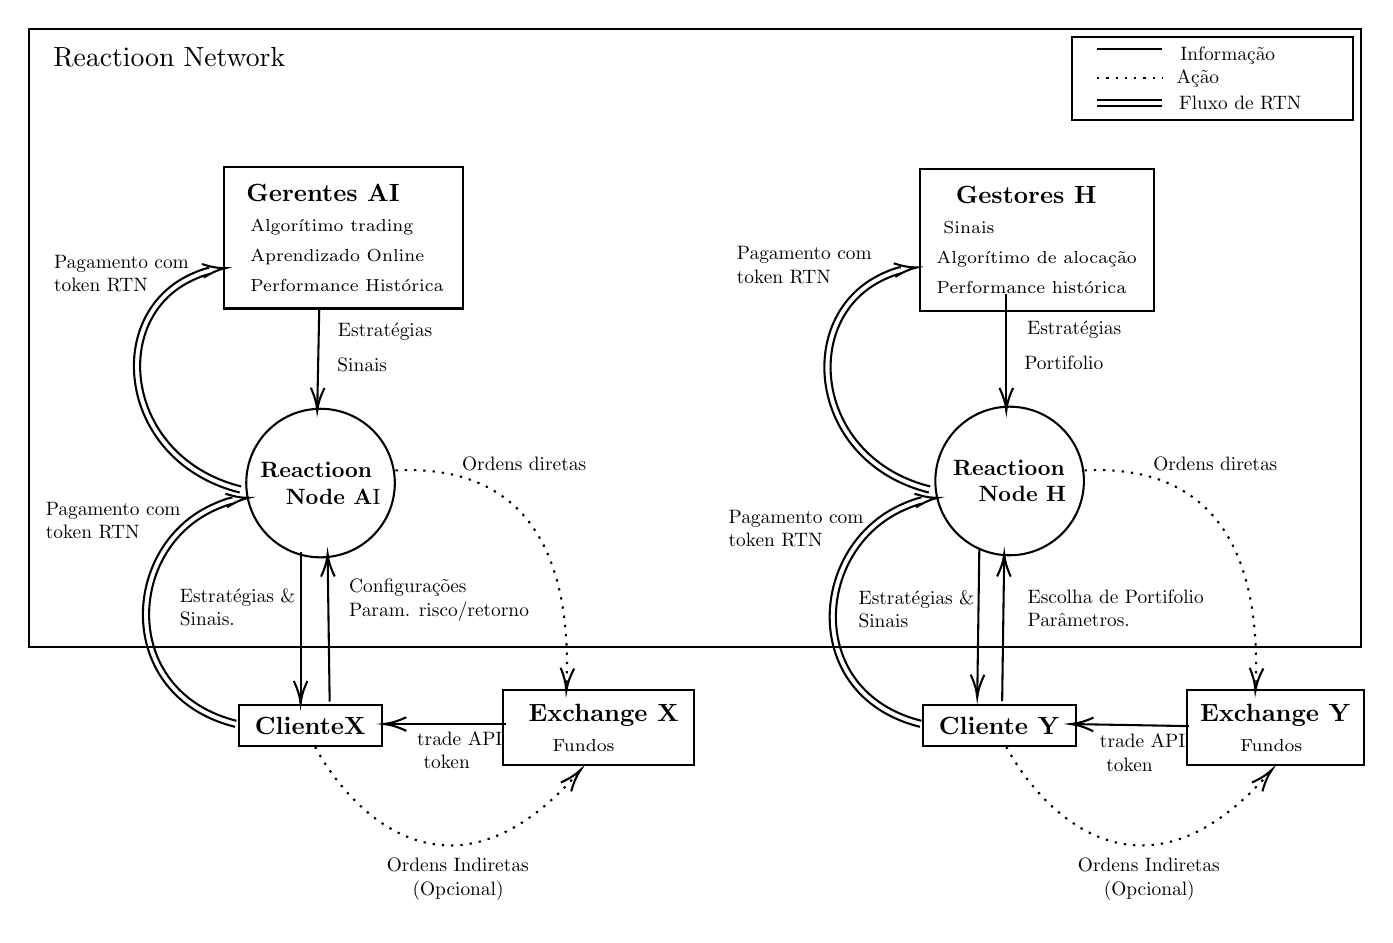
\begin{tikzpicture}[x=0.75pt,y=0.75pt,yscale=-1,xscale=1]
%uncomment if require: \path (0,464.1999969482422); %set diagram left start at 0, and has height of 464.1999969482422

%Shape: Rectangle [id:dp839607811925092] 
\draw   (16.3,16.2) -- (658.3,16.2) -- (658.3,314.2) -- (16.3,314.2) -- cycle ;
%Straight Lines [id:da3953078356379509] 
\draw    (156.3,150.2) -- (155.34,198.2) ;
\draw [shift={(155.3,200.2)}, rotate = 271.15] [color={rgb, 255:red, 0; green, 0; blue, 0 }  ][line width=0.75]    (10.93,-3.29) .. controls (6.95,-1.4) and (3.31,-0.3) .. (0,0) .. controls (3.31,0.3) and (6.95,1.4) .. (10.93,3.29)   ;

%Straight Lines [id:da5714023605084257] 
\draw    (246.3,351.2) -- (189.3,351.2) ;
\draw [shift={(187.3,351.2)}, rotate = 360] [color={rgb, 255:red, 0; green, 0; blue, 0 }  ][line width=0.75]    (10.93,-3.29) .. controls (6.95,-1.4) and (3.31,-0.3) .. (0,0) .. controls (3.31,0.3) and (6.95,1.4) .. (10.93,3.29)   ;

%Straight Lines [id:da41026468235715097] 
\draw    (161.3,340.4) -- (160.33,271.2) ;
\draw [shift={(160.3,269.2)}, rotate = 449.2] [color={rgb, 255:red, 0; green, 0; blue, 0 }  ][line width=0.75]    (10.93,-3.29) .. controls (6.95,-1.4) and (3.31,-0.3) .. (0,0) .. controls (3.31,0.3) and (6.95,1.4) .. (10.93,3.29)   ;

%Curve Lines [id:da9188372161085148] 
\draw  [dash pattern={on 0.84pt off 2.51pt}]  (193,229) .. controls (247.03,226.21) and (278.98,257.88) .. (275.36,334.05) ;
\draw [shift={(275.3,335.2)}, rotate = 272.97] [color={rgb, 255:red, 0; green, 0; blue, 0 }  ][line width=0.75]    (10.93,-3.29) .. controls (6.95,-1.4) and (3.31,-0.3) .. (0,0) .. controls (3.31,0.3) and (6.95,1.4) .. (10.93,3.29)   ;

%Curve Lines [id:da6611499345431215] 
\draw    (115.68,352.55) .. controls (92.15,346.66) and (78.57,331.56) .. (73.55,314.31) .. controls (72.05,309.15) and (71.32,303.8) .. (71.32,298.44) .. controls (71.32,298.19) and (71.32,297.93) .. (71.32,297.68) .. controls (71.58,277.85) and (81.85,258.04) .. (100.37,247.66) .. controls (106.22,244.39) and (112.89,242.05) .. (114.47,242.1)(116.41,349.64) .. controls (94.14,344.07) and (81.19,329.83) .. (76.43,313.47) .. controls (75.01,308.58) and (74.32,303.52) .. (74.32,298.44) .. controls (74.32,298.2) and (74.32,297.96) .. (74.32,297.72) .. controls (74.56,278.93) and (84.27,260.12) .. (101.84,250.28) .. controls (107.38,247.17) and (113.71,244.96) .. (114.91,245.09) ;
\draw [shift={(122.3,242.2)}, rotate = 533.23] [color={rgb, 255:red, 0; green, 0; blue, 0 }  ][line width=0.75]    (10.93,-3.29) .. controls (6.95,-1.4) and (3.31,-0.3) .. (0,0) .. controls (3.31,0.3) and (6.95,1.4) .. (10.93,3.29)   ;

%Curve Lines [id:da6558944188118099] 
\draw    (117.94,239.66) .. controls (91.22,232.98) and (75.05,214.75) .. (69.33,195.07) .. controls (68.48,192.12) and (67.85,189.14) .. (67.47,186.16) .. controls (67.14,183.68) and (66.98,181.21) .. (66.98,178.76) .. controls (66.98,161.73) and (74.72,145.63) .. (90.09,136.73) .. controls (95.48,133.61) and (101.81,131.38) .. (103.3,131.45)(118.66,236.74) .. controls (93.17,230.37) and (77.68,213.04) .. (72.22,194.23) .. controls (71.4,191.43) and (70.81,188.6) .. (70.44,185.77) .. controls (70.14,183.43) and (69.98,181.08) .. (69.98,178.76) .. controls (69.98,162.8) and (77.17,147.68) .. (91.6,139.33) .. controls (96.68,136.39) and (102.66,134.28) .. (103.68,134.45) ;
\draw [shift={(111.06,131.56)}, rotate = 533.23] [color={rgb, 255:red, 0; green, 0; blue, 0 }  ][line width=0.75]    (10.93,-3.29) .. controls (6.95,-1.4) and (3.31,-0.3) .. (0,0) .. controls (3.31,0.3) and (6.95,1.4) .. (10.93,3.29)   ;

%Curve Lines [id:da7197337789763143] 
\draw  [dash pattern={on 0.84pt off 2.51pt}]  (154.3,362.2) .. controls (173.2,397.02) and (221.81,442.74) .. (281.4,374.24) ;
\draw [shift={(282.3,373.2)}, rotate = 490.6] [color={rgb, 255:red, 0; green, 0; blue, 0 }  ][line width=0.75]    (10.93,-3.29) .. controls (6.95,-1.4) and (3.31,-0.3) .. (0,0) .. controls (3.31,0.3) and (6.95,1.4) .. (10.93,3.29)   ;

%Straight Lines [id:da7501707624311069] 
\draw    (487.3,144.2) -- (487.3,198.2) ;
\draw [shift={(487.3,200.2)}, rotate = 270] [color={rgb, 255:red, 0; green, 0; blue, 0 }  ][line width=0.75]    (10.93,-3.29) .. controls (6.95,-1.4) and (3.31,-0.3) .. (0,0) .. controls (3.31,0.3) and (6.95,1.4) .. (10.93,3.29)   ;

%Straight Lines [id:da11297405436688912] 
\draw    (575.3,352.2) -- (520.3,351.24) ;
\draw [shift={(518.3,351.2)}, rotate = 361.01] [color={rgb, 255:red, 0; green, 0; blue, 0 }  ][line width=0.75]    (10.93,-3.29) .. controls (6.95,-1.4) and (3.31,-0.3) .. (0,0) .. controls (3.31,0.3) and (6.95,1.4) .. (10.93,3.29)   ;

%Straight Lines [id:da9530469398494208] 
\draw    (485.3,340.2) -- (486.27,271.2) ;
\draw [shift={(486.3,269.2)}, rotate = 450.81] [color={rgb, 255:red, 0; green, 0; blue, 0 }  ][line width=0.75]    (10.93,-3.29) .. controls (6.95,-1.4) and (3.31,-0.3) .. (0,0) .. controls (3.31,0.3) and (6.95,1.4) .. (10.93,3.29)   ;

%Curve Lines [id:da6669727888364709] 
\draw  [dash pattern={on 0.84pt off 2.51pt}]  (525,229) .. controls (579.03,226.21) and (610.98,257.88) .. (607.36,334.05) ;
\draw [shift={(607.3,335.2)}, rotate = 272.97] [color={rgb, 255:red, 0; green, 0; blue, 0 }  ][line width=0.75]    (10.93,-3.29) .. controls (6.95,-1.4) and (3.31,-0.3) .. (0,0) .. controls (3.31,0.3) and (6.95,1.4) .. (10.93,3.29)   ;

%Curve Lines [id:da6929077991045711] 
\draw    (445.68,352.55) .. controls (422.54,346.76) and (409.27,332.05) .. (404.37,315.16) .. controls (402.91,310.12) and (402.2,304.87) .. (402.2,299.6) .. controls (402.2,298.95) and (402.21,298.3) .. (402.23,297.65) .. controls (402.9,277.57) and (413.86,257.51) .. (433.02,247.25) .. controls (438.74,244.19) and (445.19,242) .. (446.5,242.09)(446.41,349.64) .. controls (424.53,344.17) and (411.89,330.33) .. (407.26,314.33) .. controls (405.87,309.55) and (405.2,304.59) .. (405.2,299.6) .. controls (405.2,298.98) and (405.21,298.36) .. (405.23,297.75) .. controls (405.86,278.7) and (416.25,259.64) .. (434.43,249.9) .. controls (439.87,246.99) and (445.99,244.92) .. (446.94,245.08) ;
\draw [shift={(454.3,242.2)}, rotate = 533.23] [color={rgb, 255:red, 0; green, 0; blue, 0 }  ][line width=0.75]    (10.93,-3.29) .. controls (6.95,-1.4) and (3.31,-0.3) .. (0,0) .. controls (3.31,0.3) and (6.95,1.4) .. (10.93,3.29)   ;

%Curve Lines [id:da46112590181388846] 
\draw    (449.94,239.66) .. controls (423.51,233.05) and (407.61,215.09) .. (401.97,195.59) .. controls (401.05,192.4) and (400.4,189.18) .. (400.03,185.95) .. controls (399.77,183.73) and (399.64,181.5) .. (399.64,179.29) .. controls (399.64,162) and (407.53,145.57) .. (423.1,136.49) .. controls (428.56,133.31) and (434.97,131.03) .. (436.48,131.11)(450.66,236.74) .. controls (425.47,230.45) and (410.24,213.37) .. (404.85,194.75) .. controls (403.98,191.73) and (403.36,188.67) .. (403.01,185.61) .. controls (402.76,183.5) and (402.64,181.39) .. (402.64,179.29) .. controls (402.64,163.07) and (409.98,147.61) .. (424.62,139.09) .. controls (429.77,136.08) and (435.82,133.94) .. (436.95,134.08) ;
\draw [shift={(444.3,131.2)}, rotate = 533.23] [color={rgb, 255:red, 0; green, 0; blue, 0 }  ][line width=0.75]    (10.93,-3.29) .. controls (6.95,-1.4) and (3.31,-0.3) .. (0,0) .. controls (3.31,0.3) and (6.95,1.4) .. (10.93,3.29)   ;

%Curve Lines [id:da8354818907327548] 
\draw  [dash pattern={on 0.84pt off 2.51pt}]  (487.3,362.2) .. controls (506.2,397.02) and (554.81,442.74) .. (614.4,374.24) ;
\draw [shift={(615.3,373.2)}, rotate = 490.6] [color={rgb, 255:red, 0; green, 0; blue, 0 }  ][line width=0.75]    (10.93,-3.29) .. controls (6.95,-1.4) and (3.31,-0.3) .. (0,0) .. controls (3.31,0.3) and (6.95,1.4) .. (10.93,3.29)   ;

%Straight Lines [id:da8770926699692774] 
\draw    (147.3,268.2) -- (147.3,339.4) ;
\draw [shift={(147.3,341.4)}, rotate = 270] [color={rgb, 255:red, 0; green, 0; blue, 0 }  ][line width=0.75]    (10.93,-3.29) .. controls (6.95,-1.4) and (3.31,-0.3) .. (0,0) .. controls (3.31,0.3) and (6.95,1.4) .. (10.93,3.29)   ;

%Straight Lines [id:da36937072037759555] 
\draw    (474.3,267.2) -- (473.33,336.4) ;
\draw [shift={(473.3,338.4)}, rotate = 270.8] [color={rgb, 255:red, 0; green, 0; blue, 0 }  ][line width=0.75]    (10.93,-3.29) .. controls (6.95,-1.4) and (3.31,-0.3) .. (0,0) .. controls (3.31,0.3) and (6.95,1.4) .. (10.93,3.29)   ;

%Shape: Rectangle [id:dp03825033305531944] 
\draw   (518.9,20) -- (654.3,20) -- (654.3,60) -- (518.9,60) -- cycle ;
%Straight Lines [id:da5606203321141707] 
\draw    (531,26) -- (562.3,26) ;


%Straight Lines [id:da21375108102279738] 
\draw  [dash pattern={on 0.84pt off 2.51pt}]  (531,40) -- (562.3,40) ;


%Straight Lines [id:da15988012489637837] 
\draw    (531,50.5) -- (562.3,50.5)(531,53.5) -- (562.3,53.5) ;



% Text Node
\draw    (245,335) -- (337,335) -- (337,371) -- (245,371) -- cycle  ;
\draw (291,353) node [scale=0.9] [align=left] {\textbf{ Exchange X }\\{\scriptsize  \ \ \ \ \ Fundos}};
% Text Node
\draw    (117.5,342) -- (186.5,342) -- (186.5,362) -- (117.5,362) -- cycle  ;
\draw (152,352) node [scale=0.9] [align=left] {\textbf{ ClienteX }};
% Text Node
\draw    (110.5,83) -- (225.5,83) -- (225.5,151) -- (110.5,151) -- cycle  ;
\draw (168,117) node [scale=0.9] [align=left] {\textbf{ Gerentes AI}\\{\scriptsize  \ \ Algorítimo trading}\\{\scriptsize  \ \ Aprendizado Online \ }\\{\scriptsize  \ \ Performance Histórica \ }};
% Text Node
\draw    (156.9, 235.1) circle [x radius= 35.79, y radius= 35.79]   ;
\draw (156.9,235.1) node [scale=0.8] [align=left] {\textbf{Reactioon}\\\textbf{ \ \ Node A}I};
% Text Node
\draw (84,30) node  [align=left] {Reactioon Network};
% Text Node
\draw (224,364) node [scale=0.7] [align=left] {trade API \\ \ token};
% Text Node
\draw (188,162) node [scale=0.7] [align=left] {Estratégias};
% Text Node
\draw (177,178) node [scale=0.7] [align=left] {Sinais};
% Text Node
\draw (214,296) node [scale=0.7] [align=left] {Configurações\\Param. risco/retorno\\};
% Text Node
\draw (61,134) node [scale=0.7] [align=left] {Pagamento com\\ token RTN};
% Text Node
\draw (255,226) node [scale=0.7] [align=left] {Ordens diretas};
% Text Node
\draw (223,426) node [scale=0.7] [align=left] {Ordens Indiretas\\ \ \ \ \ (Opcional)};
% Text Node
\draw    (574.5,335) -- (659.5,335) -- (659.5,371) -- (574.5,371) -- cycle  ;
\draw (617,353) node [scale=0.9] [align=left] {\textbf{Exchange Y}\\{\scriptsize  \ \ \ \ \ \ Fundos}};
% Text Node
\draw    (447,342) -- (521,342) -- (521,362) -- (447,362) -- cycle  ;
\draw (484,352) node [scale=0.9] [align=left] {\textbf{ Cliente Y }};
% Text Node
\draw    (445.5,84) -- (558.5,84) -- (558.5,152) -- (445.5,152) -- cycle  ;
\draw (502,118) node [scale=0.9] [align=left] {\textbf{ \ Gestores H}\\{\scriptsize  \ Sinais}\\ {\scriptsize Algorítimo de alocação \ }\\{\scriptsize  Performance histórica }};
% Text Node
\draw    (488.9, 234.1) circle [x radius= 35.79, y radius= 35.79]   ;
\draw (488.9,234.1) node [scale=0.8] [align=left] {\textbf{Reactioon}\\\textbf{ \ \ Node H}};
% Text Node
\draw (540,301) node [scale=0.7] [align=left] {Escolha de Portifolio\\Parâmetros.\\};
% Text Node
\draw (588,226) node [scale=0.7] [align=left] {Ordens diretas};
% Text Node
\draw (117,306) node [scale=0.7] [align=left] {Estratégias \&\\Sinais.\\\\};
% Text Node
\draw (444,307) node [scale=0.7] [align=left] {Estratégias \&\\Sinais\\\\};
% Text Node
\draw (579.6,40) node [scale=0.7] [align=left] {Ação};
% Text Node
\draw (594,29) node [scale=0.7] [align=left] {Informação};
% Text Node
\draw (600,52) node [scale=0.7] [align=left] {Fluxo de RTN};
% Text Node
\draw (553,365) node [scale=0.7] [align=left] {trade API \\ \ token};
% Text Node
\draw (390,130) node [scale=0.7] [align=left] {Pagamento com\\ token RTN};
% Text Node
\draw (520,161) node [scale=0.7] [align=left] {Estratégias};
% Text Node
\draw (515,177) node [scale=0.7] [align=left] {Portifolio};
% Text Node
\draw (57,253) node [scale=0.7] [align=left] {Pagamento com\\ token RTN};
% Text Node
\draw (386,257) node [scale=0.7] [align=left] {Pagamento com\\ token RTN};
% Text Node
\draw (556,426) node [scale=0.7] [align=left] {Ordens Indiretas\\ \ \ \ \ (Opcional)};


\end{tikzpicture}
